% G3 release paper (v3.0.0+). Every quantity comes from generated/*.tex, which `g3-release-tex` writes from the
% committed release receipt evidence/g3/v<VERSION>/release.json; build with `make -C docs/g3/paper`.
\documentclass[10pt,journal,letterpaper]{IEEEtran}
\usepackage{amsmath,amssymb,graphicx,booktabs,array,xcolor,url}
% ei-ieee-skin.tex -- "research skin" for the IEEEtran journal build of both papers and the supplement.
% Load AFTER amsmath/amssymb and BEFORE hyperref. LuaLaTeX only (fontspec + unicode-math).
% Termes body and matching Termes Math at IEEE's 10/12, so the page count is unchanged (measured in the
% paper study of 2026-10-25); sans headings, captions and tables; one callout style; slate running heads.
\usepackage{fontspec}
\usepackage[math-style=TeX,bold-style=TeX]{unicode-math}
\setmainfont{TeX Gyre Termes}\setmathfont{TeX Gyre Termes Math}% same metrics as before; math now matches text
\setsansfont{TeX Gyre Heros}[Scale=0.94]
\setmonofont{DejaVu Sans Mono}[Scale=0.80]% heavier, more legible identifiers than Cursor
\usepackage{xcolor,etoolbox}
\definecolor{ink}{HTML}{132D3B}\definecolor{teal}{HTML}{007E87}\definecolor{rust}{HTML}{A3442D}
\definecolor{hair}{HTML}{D3D9DF}\definecolor{slate}{HTML}{5B6773}\definecolor{tealpale}{HTML}{EAF4F5}
% ---- headings: sans bold ink, teal arabic numbers (IEEE roman numerals and small caps dropped)
\makeatletter
\def\thesection{\arabic{section}}
\def\thesubsection{\thesection.\arabic{subsection}}
\def\thesectiondis{{\color{teal}\thesection}}
\def\thesubsectiondis{{\color{teal}\thesection.\arabic{subsection}}}
\def\thesubsubsectiondis{}
\def\@seccntformat#1{\csname the#1dis\endcsname\hskip 0.55em\relax}
\def\section{\@startsection{section}{1}{\z@}{2.1ex plus 1ex minus 0.4ex}{0.7ex plus 0.2ex}%
  {\normalfont\sffamily\bfseries\fontsize{10.4}{12.4}\selectfont\color{ink}\raggedright}}
\def\subsection{\@startsection{subsection}{2}{\z@}{1.5ex plus 0.7ex minus 0.3ex}{0.4ex plus 0.2ex}%
  {\normalfont\sffamily\bfseries\fontsize{9}{11}\selectfont\color{ink}\raggedright}}
\def\subsubsection{\@startsection{subsubsection}{3}{\z@}{1ex plus .4ex minus .2ex}{-0.6em}%
  {\normalfont\sffamily\bfseries\fontsize{8.6}{10.4}\selectfont\color{ink}}}
% ---- captions: sans 7.6/9.6, bold ink label, teal bar separator, ragged right, table caption above
\def\figurename{Figure}\def\tablename{Table}\def\thetable{\arabic{table}}
\def\fnum@table{\tablename~\thetable}
\newcommand{\EIcapsep}{\enspace{\color{teal}\rule[-0.2ex]{0.6pt}{1.9ex}}\enspace}
\long\def\@makecaption#1#2{%
  \ifx\@captype\@IEEEtablestring
    \bgroup\par\raggedright\@IEEEtabletopskipstrut{\sffamily\fontsize{7.6}{9.6}\selectfont{\bfseries\color{ink}#1}\EIcapsep #2\par}\addvspace{0.45\baselineskip}\egroup
    \@IEEEtablecaptionsepspace
  \else
    \@IEEEfigurecaptionsepspace
    \parbox[t]{\hsize}{\sffamily\fontsize{7.6}{9.6}\selectfont\raggedright{\bfseries\color{ink}#1}\EIcapsep #2}%
  \fi}
\makeatother
% ---- tables: sans 7.8/9.8 everywhere (sections' \small inside tables is mapped to it), ink rules
\newcommand{\EItablefont}{\sffamily\fontsize{7.8}{9.8}\selectfont}
\makeatletter% IEEEtran's \table resets to \footnotesize inside the float box; reset to the sans table face instead
\def\table{\def\@floatboxreset{\reset@font\EItablefont\let\small\EItablefont\@setminipage}\@float{table}}
\@namedef{table*}{\def\@floatboxreset{\reset@font\EItablefont\let\small\EItablefont\@setminipage}\@dblfloat{table}}
\makeatother
\AtBeginDocument{\setlength{\heavyrulewidth}{0.7pt}\setlength{\lightrulewidth}{0.35pt}}
% ---- identifiers: xurl lets \nolinkurl stretch between characters in justified text; keep it near rigid
\AtBeginDocument{\Urlmuskip=0mu plus 0.1mu}
% ---- one callout style (scope / claims boxes)
\RequirePackage[most]{tcolorbox}
\newtcolorbox{eibox}[1]{enhanced,breakable,colback=tealpale,colframe=teal,boxrule=0pt,leftrule=1.8pt,
  arc=0pt,outer arc=0pt,left=5pt,right=5pt,top=4pt,bottom=4pt,
  fontupper=\sffamily\fontsize{7.8}{10}\selectfont\color{ink},
  title={\sffamily\bfseries\fontsize{8}{10}\selectfont #1},coltitle=teal!70!black,colbacktitle=tealpale,
  attach title to upper={\par\vspace{1.5pt}},before skip=7pt,after skip=7pt}
% ---- running heads: sans, letterspaced, slate
\RequirePackage{fancyhdr}
\fancypagestyle{headings}{\fancyhf{}\renewcommand{\headrulewidth}{0pt}%
  \fancyhead[L]{\sffamily\fontsize{6.6}{8}\selectfont\color{slate}\addfontfeature{LetterSpace=8}ENGINEERED INTELLIGENCE\enspace{\color{hair}|}\enspace\addfontfeature{LetterSpace=0}Tracing computational design from search to evidence}%
  \fancyhead[R]{\sffamily\fontsize{6.6}{8}\selectfont\color{slate}\thepage}}
% ---- numbers: generated counts are typeset with \num{} (thousands grouped); commas in input are ignored
\RequirePackage{siunitx}
\sisetup{group-separator={,}, group-minimum-digits=4, input-decimal-markers={.}, input-ignore={,}, mode=text, reset-text-family=false, reset-text-series=false}
% ---- page-1 furniture: kicker row and key-number tiles (values only from generated macros)
\newcommand{\kicker}[1]{{\sffamily\fontsize{6.8}{8}\selectfont\addfontfeature{LetterSpace=9}#1}}
\newcommand{\stat}[2]{\begin{minipage}[t]{0.18\textwidth}\raggedright
  {\sffamily\bfseries\fontsize{14}{16}\selectfont\color{ink}#1}\par\vspace{2pt}
  {\sffamily\fontsize{6.8}{8.4}\selectfont\color{slate}#2}\end{minipage}}
% ---- chart tokens (dataviz reference instance; categorical slots 1-3 validated all-pairs on white) and chrome
\definecolor{seriesA}{HTML}{2A78D6}\definecolor{seriesB}{HTML}{EB6834}\definecolor{seriesC}{HTML}{1BAF7A}
\definecolor{gridgray}{HTML}{E1E0D9}\definecolor{axisgray}{HTML}{C3C2B7}

\usepackage{xurl}
\usepackage[hidelinks]{hyperref}
\usepackage{microtype}
% generated by g3-release-tex from evidence/g3/v<VERSION>/release.json; do not edit
\newcommand{\gVersion}{3.0.1}
\newcommand{\gRecord}{3.0.0}
\newcommand{\gDesign}{\texttt{hz4i013\_g00995\_d206e3c9}}
\newcommand{\gStatus}{computational design; not built, printed or physically tested}
\newcommand{\gCommit}{\texttt{80e669e5b558}}
\newcommand{\gDecoder}{\texttt{a203278d80d2}}
\newcommand{\gGenomeSha}{\texttt{d206e3c9f4c3}}
\newcommand{\gMetric}{W\_ERGOLIGHT\_v1 draft d}
\newcommand{\gPlatform}{Linux x86\_64 (xbabe2), Tier 2 at h 0.2 mm}
\newcommand{\gScore}{80.55}
\newcommand{\gBase}{0.815}
\newcommand{\gE}{0.988}
\newcommand{\gScoreArm}{80.55}
\newcommand{\gMassG}{59.3}
\newcommand{\gMassVoxelG}{56.0}
\newcommand{\gVolAM}{13,385}
\newcommand{\gVolEnv}{26,954}
\newcommand{\gDensity}{0.00443}
\newcommand{\gIslands}{24}
\newcommand{\gEvalsIsland}{2,500}
\newcommand{\gEvalsIslandRaw}{2500}
\newcommand{\gEvalsTotal}{60,000}
\newcommand{\gElites}{3,177}
\newcommand{\gTierTwo}{68}
\newcommand{\gGateOne}{62}
\newcommand{\gGateTwo}{71}
\newcommand{\gH}{0.4}
\newcommand{\gHRank}{0.2}
\newcommand{\gMassRankG}{57.0}
\newcommand{\gScoreSearch}{80.77}
\newcommand{\gLeader}{\texttt{hz4i013\_g00840\_2a44149e}}
\newcommand{\gLeaderTierTwo}{81.53}
\newcommand{\gLeaderMassA}{51.3}
\newcommand{\gLeaderMassB}{75.2}
\newcommand{\gLeaderMassC}{74.6}
\newcommand{\gGridAgree}{3.3}
\newcommand{\gLeaderScoreA}{75.06}
\newcommand{\gLeaderScoreB}{66.65}
\newcommand{\gHost}{xbabe4 (arm64 macOS)}
\newcommand{\gStarted}{2026-10-26T11:03:49Z}
\newcommand{\gFinished}{2026-10-26T12:32:55Z}
\newcommand{\gWinIsland}{island13}
\newcommand{\gScoreSobol}{56.54}
\newcommand{\gTipSF}{0.64}
\newcommand{\gGripSF}{0.73}
\newcommand{\gLatN}{337}
\newcommand{\gHmTwist}{1.09}
\newcommand{\gHmSpine}{1.44}
\newcommand{\gFat}{0.94}
\newcommand{\gSeq}{0.56}
\newcommand{\gBuck}{11.2}
\newcommand{\gRingBear}{8,677}
\newcommand{\gRingBack}{1,686}
\newcommand{\gLg}{64.9}
\newcommand{\gSwellPerim}{64.4}
\newcommand{\gHoT}{1.59}
\newcommand{\gComIdx}{7.0}
\newcommand{\gGuardH}{11.4}
\newcommand{\gApexMax}{0.092}
\newcommand{\gHalfAngleMax}{21.7}
\newcommand{\gReach}{69.3}
\newcommand{\gToothSnag}{180}
\newcommand{\gToothPry}{60}
\newcommand{\gFeAllow}{674}
\newcommand{\gFeH}{0.4}
\newcommand{\gFeGripLat}{3.55}
\newcommand{\gFeGripTwist}{5.50}
\newcommand{\gFeGripSpine}{0.74}
\newcommand{\gFeRootLat}{2.08}
\newcommand{\gFeRootTwist}{1.69}
\newcommand{\gFeRootSpine}{1.29}
\newcommand{\gFormLat}{5.07}
\newcommand{\gFormTwist}{12.69}
\newcommand{\gFormSpine}{0.90}
\newcommand{\gTipConvA}{0.585}
\newcommand{\gTipConvB}{0.638}
\newcommand{\gTipConvC}{0.611}
\newcommand{\gEdgeAApexLo}{20.5}
\newcommand{\gEdgeAApexHi}{20.8}
\newcommand{\gEdgeABevelLo}{19.5}
\newcommand{\gEdgeABevelHi}{20.8}
\newcommand{\gEdgeASteep}{20.9}
\newcommand{\gEdgeAFrom}{57.0}
\newcommand{\gEdgeATo}{3.0}
\newcommand{\gEdgeAPlunge}{9.7}
\newcommand{\gEdgeADepth}{1.63}
\newcommand{\gEdgeATeeth}{3}
\newcommand{\gEdgeATeethChecked}{2}
\newcommand{\gEdgeAToothSF}{3.47}
\newcommand{\gEdgeAFlank}{39}
\newcommand{\gEdgeAArc}{67.1}
\newcommand{\gEdgeASharpened}{60.7}
\newcommand{\gEdgeBApexLo}{20.6}
\newcommand{\gEdgeBApexHi}{21.6}
\newcommand{\gEdgeBBevelLo}{18.7}
\newcommand{\gEdgeBBevelHi}{21.7}
\newcommand{\gEdgeBSteep}{21.9}
\newcommand{\gEdgeBFrom}{65.1}
\newcommand{\gEdgeBTo}{3.1}
\newcommand{\gEdgeBPlunge}{11.9}
\newcommand{\gEdgeBDepth}{1.41}
\newcommand{\gEdgeBTeeth}{5}
\newcommand{\gEdgeBTeethChecked}{4}
\newcommand{\gEdgeBToothSF}{2.83}
\newcommand{\gEdgeBFlank}{36}
\newcommand{\gEdgeBArc}{77.3}
\newcommand{\gEdgeBSharpened}{69.5}
\newcommand{\gMassReading}{is above the 50 g goal}
\newcommand{\gTipReading}{is below the target}
\newcommand{\gGripReading}{is below the target}
\newcommand{\gTwistReading}{meets the target}
\newcommand{\gSpineReading}{meets the target}
\newcommand{\gToothReading}{meets the target}
\newcommand{\gToothMin}{2.83}
\newcommand{\gFatReading}{is below the target}
\newcommand{\gSeqReading}{is below the target}
\newcommand{\gLatReading}{meets the target}
\newcommand{\gRingReading}{meets the target}
\newcommand{\gBuckReading}{meets the target}
\graphicspath{{../v3.0.0/img/}}
\newcommand{\gTopEightRows}{%
1 & \texttt{hz4i013\_g00995\_d206e3c9} & 80.55 & 57.0 \\
2 & \texttt{hz4i002\_g00995\_6f4643f1} & 80.44 & 58.7 \\
3 & \texttt{hz4i013\_g00345\_be45c4bc} & 79.51 & 56.7 \\
4 & \texttt{hz4i002\_g00479\_76f5e0ac} & 79.39 & 59.5 \\
5 & \texttt{hz4i013\_g00555\_5cd1f106} & 79.27 & 52.1 \\
6 & \texttt{hz4i004\_g00501\_cb3c9e4e} & 79.24 & 57.3 \\
7 & \texttt{hz4i002\_g00905\_b274d4d9} & 78.94 & 59.6 \\
8 & \texttt{hz4i007\_g00005\_98a9344b} & 78.77 & 53.7 \\}
\newcommand{\gAssetRows}{%
\texttt{AMbuild\_mm.stl} & 1,001,372 & 48 & git and release \\
\texttt{envelope\_mm.stl} & 911,132 & 43 & git and release \\
\texttt{AMbuild\_h0.2\_mm.stl} & 5,373,548 & 256 & release \\
\texttt{envelope\_h0.2\_mm.stl} & 2,063,960 & 98 & release \\
\texttt{envelope\_fineblade\_mm.stl} & 3,843,106 & 183 & release \\}
\newcommand{\gGridRows}{%
\texttt{hz4i013\_g00840\_2a44149e} & 51.3 & 55.6 & 54.9 & 75.2 & 74.6 \\
\texttt{hz4i013\_g00995\_d206e3c9} & 56.0 & 60.0 & 59.0 & 57.0 & 57.5 \\
\texttt{hz4i002\_g00995\_6f4643f1} & 58.8 & 59.6 & 58.9 & 58.7 & 58.5 \\
\texttt{hz4i013\_g00345\_be45c4bc} & 55.3 & 59.7 & 56.4 & 56.7 & 57.1 \\
\texttt{hz4i002\_g00479\_76f5e0ac} & 58.0 & 61.7 & 58.2 & 59.5 & 58.9 \\
\texttt{hz4i013\_g00555\_5cd1f106} & 50.6 & 54.1 & 54.4 & 52.1 & 53.1 \\
\texttt{hz4i005\_g00345\_c7922cf1} & 56.8 & 61.0 & 57.6 & 58.5 & 59.7 \\
\texttt{hz4i002\_g00785\_6b2ff4aa} & 59.1 & 62.0 & 58.8 & 61.8 & 59.8 \\}

\hypersetup{
  pdftitle={Evolving a printable titanium karambit under ergonomic, edge and serration constraints (G3 v\gVersion)},
  pdfauthor={Jepson Taylor},
  pdflang={en-US},
  pdfkeywords={evolutionary design, quality diversity, MAP-Elites, additive manufacturing, Ti-6Al-4V, finite elements, knife design}
}
\DeclareRobustCommand{\code}[1]{\texorpdfstring{{\nolinkurl{#1}}}{#1}}
\newcommand{\src}[2]{\href{https://github.com/neverhuman/jarambit/blob/v\gVersion/#1}{#2}}
\makeatletter
\fancypagestyle{headings}{\fancyhf{}\renewcommand{\headrulewidth}{0pt}%
  \fancyhead[L]{\sffamily\fontsize{6.6}{8}\selectfont\color{slate}\addfontfeature{LetterSpace=8}JARAMBIT G3\enspace{\color{hair}|}\enspace\addfontfeature{LetterSpace=0}An evolved, printable titanium karambit (v\gVersion)}%
  \fancyhead[R]{\sffamily\fontsize{6.6}{8}\selectfont\color{slate}\thepage}}
\makeatother
\pagestyle{headings}

\begin{document}
\title{Evolving a Printable Titanium Karambit under Ergonomic, Edge and Serration Constraints}
\author{Jepson Taylor%
\thanks{Release v\gVersion, decoder commit \gCommit{} (decoder hash \gDecoder). All figures and numbers in this paper
are generated from the release receipt \code{evidence/g3/v\gVersion/release.json}. Status: \gStatus.}}
\maketitle

\begin{abstract}
We report the best individual of the G3 v\gVersion{} cohort of record, a one-piece Ti-6Al-4V karambit for laser
powder-bed fusion with a hollow, lattice-filled grip and blade core. No person designed it: \gIslands{} independent
CVT-MAP-Elites islands ran \gEvalsIsland{} evaluations each from scrambled Sobol samples, and the design space itself
carries the rules a good edge must follow. Both cutting edges have one primary grind of
\gEdgeAApexLo--\gEdgeAApexHi\textdegree{} and \gEdgeBApexLo--\gEdgeBApexHi\textdegree{} per side, measured normal to
the edge and carried to within \gEdgeATo{} and \gEdgeBTo{} mm of the point, and both edges are serrated
(\gEdgeATeeth{} and \gEdgeBTeeth{} teeth; the weakest tooth has a safety factor of \gToothMin{} under a
\gToothSnag{} N snag). The design scores \gScore{} under \gMetric{} with an ergonomic multiplier of \gE{} and
weighs \gMassG{} g as printed, which \gMassReading. The \gH{} mm search grid undercounted the mass of the
search's own leader (\gLeaderMassA{} g against \gLeaderMassB{} g at 0.2 mm and \gLeaderMassC{} g at 0.15 mm), so the
ranking of record is measured on
the \gHRank{} mm grid of the print file. Against a safety-factor target of 1, its solid tip
(\gTipSF) \gTipReading{} and its grip under the spine load (\gFeGripSpine{} by voxel FE) \gGripReading. We describe
the representation, objective, search and measurement chain, the evolution that produced the design, and every limit
of the result.
\end{abstract}

\begin{IEEEkeywords}
Evolutionary design, quality diversity, MAP-Elites, additive manufacturing, Ti-6Al-4V, finite elements, knife design.
\end{IEEEkeywords}

\section{Introduction}\label{sec:intro}
A karambit is a curved, ring-retained utility and defensive knife gripped in a closed fist with the index or little
finger seated through a rear retention ring. Fabricating a one-piece karambit in Ti-6Al-4V by laser powder-bed fusion
(L-PBF) opens an expressive three-dimensional design space: the grip and blade core can be hollowed into a skin over a
triply periodic minimal-surface (TPMS) lattice with integral powder-evacuation ports, while variable-thickness ribs,
finger grooves and dual-edge bevels are built directly into the single monolithic part. Yet unrestricted evolutionary
search in three dimensions also creates severe specification traps. A coarse voxel grid can hide mass or bridge thin
gaps; a beam or plate surrogate can credit interior material that is absent from the printed build; a blade profile can
leave an unground shoulder where a sparse station check does not look; and deep, narrow serration gullets can inflate
apparent edge length while leaving brittle needle teeth that snap under an oblique snag.

Generation~3 (G3) of the Jarambit project addresses these failure modes by formulating the whole knife---retention
ring, ergonomic grip, guard, hollow lattice interior, and a double-edged, double-serrated claw blade---inside a unified
constructive decoder and multi-fidelity finite-element evaluation pipeline. This paper reports the v\gVersion{} release
and the best individual of its cohort of record, \gDesign{} (commit \gCommit, decoder hash \gDecoder).

Three architectural principles govern the v\gVersion{} release:
\begin{enumerate}
\item \emph{Evolution designs the knife from scratch.} Every island in the cohort is initialised exclusively from
scrambled low-discrepancy Sobol sequences (\src{crates/g3/src/g3_genome.rs}{\code{g3_genome.rs}}). No hand-tuned seed,
template CAD model or post-hoc manual edit enters the population. Engineering laws are encoded either as invariant
geometric mappings inside the decoder or as measured physical responses in the objective.
\item \emph{Edge and serration mechanics are intrinsic to the decoder.} Rather than treating sharpening and serrations
as a post-process applied after structural optimisation, decoder revision~r2 enforces five primary-grind invariants
(EDGE-1..5) and four serration-integrity laws (SERR-1..4) directly on the signed distance field
(\src{crates/g3/src/g3_sdf.rs}{\code{g3_sdf.rs}}; Section~\ref{sec:design}). Both cutting edges carry a single primary
bevel at a titanium-appropriate angle (17.5--22.5\textdegree{} per side) measured normal to the true serrated edge
curve, run unbroken to the piercing point, and carry scalloped serrations whose individual tooth roots are checked
against combined in-plane snag (\gToothSnag~N) and cross-blade pry (\gToothPry~N) loads
(\src{crates/g3/src/g3_qd.rs}{\code{serration_tooth_strength}}).
\item \emph{Every reported quantity traces to a single committed measurement receipt.} All scores, dimensions, safety
factors, convergence checks and rankings in this paper and in the repository \code{README.md} are generated
automatically from \code{evidence/g3/v\gVersion/release.json} via
\src{crates/g3/src/bin/g3_release_tex.rs}{\code{g3_release_tex.rs}} and \src{ops/ci/gen_readme.py}{\code{gen_readme.py}}.
Analytic Tier-0 screening estimates never appear in reported results; every quoted value comes from voxel-SDF geometry,
plate and solid finite elements, and an explicit \code{hex8} voxel finite-element certification of the printed part.
\end{enumerate}

The remainder of this paper details the 179-gene representation and edge/serration decoder laws
(Section~\ref{sec:design}), the veto-free multiplicative-ergonomics objective \gMetric{} (Section~\ref{sec:objective}),
the \gIslands-island CVT-MAP-Elites search and three-tier evaluation cascade (Section~\ref{sec:search}), the
multi-grid and voxel finite-element verification chain (Section~\ref{sec:measure}), the evolutionary trajectory and
best individual \gDesign{} (Section~\ref{sec:results}), the explicit physical and modelling limits of the result
(Section~\ref{sec:limits}), and the complete reproduction protocol (Section~\ref{sec:repro}).

\section{Design space}\label{sec:design}
\subsection{Genome and decoder}
A G3.0 genome is 179 real genes in the unit cube (\src{crates/g3/src/g3_genome.rs}{\code{g3_genome.rs}}). The decoder
maps them to physical parameters and builds a signed distance field (SDF) of the whole knife
(\src{crates/g3/src/g3_sdf.rs}{\code{g3_sdf.rs}}): a finger ring with a fixed 24.9 mm bore and 8 mm lip, a compact grip
with finger grooves and a textured surface, a guard, and a curved claw blade whose straight-line reach from the guard
is capped at 85.725 mm. The interior of the grip and blade is a skin over a triply periodic minimal-surface lattice
with powder-removal ports, so the part can be printed hollow. The decoder revision of this release, r2, is identified by
the hash \gDecoder{} of its source files; an archive made under another decoder fails its integrity check.

\subsection{Edge rules (EDGE-1..5)}
Each cutting edge has one primary grind whose per-side angle is a gene bounded to 17.5--22.5\textdegree{} (35--45\textdegree{}
inclusive, centred on 20\textdegree{} as a hard-use edge for titanium). The bevel depth is the true distance to the
actual, serrated edge polyline, so the angle is the same on the curved claw as on the straight part, and the grind is
carried at full height until it meets the blade body, with no micro-bevel and no shoulder (EDGE-1, -2, -3). Both grinds
run unbroken to the point; only a plunge of 5--12\,\% of the edge length next to the guard is unsharpened, inside a
4.0\,in sharpened-length cap per edge (EDGE-4). The sharpness check reads the true edge-normal section over the first
2 mm at every steady station, so a shoulder behind the apex would cost score (EDGE-5).

\subsection{Serration rules (SERR-1..4)}
Both edges are serrated. The serration depth is 0.8--2.2 mm on the inner edge and 0.8--2.0 mm on the spine edge
(SERR-1); every serrated span holds at least three full-depth teeth (SERR-2); the span starts past the plunge and ends at
least 18 mm from the point, so the piercing point stays plain (SERR-3). To keep teeth from snapping, the pitch is
5--9 mm and the depth is at most a quarter of the pitch (SERR-4). Each tooth is checked as built
(\src{crates/g3/src/g3_qd.rs}{\code{serration_tooth_strength}}): its root is the segment between two neighbouring gullet
bottoms, with the thickness of the exact blade law along it; a \gToothSnag{} N snag along the edge, amplified by the
Inglis notch factor $K_t = 1 + 2\sqrt{d/\rho}$ for gullet depth $d$ and radius $\rho$~\cite{inglis1913}, and a
\gToothPry{} N pry across the blade load the tooth tip. The decoder test suite requires every tooth of 60 Sobol designs
to reach a safety factor of at least 1 under both cases.

\section{Objective}\label{sec:objective}
Candidates are ranked by the veto-free continuous objective \code{W\_ERGOLIGHT\_v1} (draft~d, requirement set
\code{RS-karambit-v3}; \src{crates/g3/src/ergolight.rs}{\code{ergolight.rs}}):
\begin{equation}
\mathrm{score}_{100} = 100\,E \sum_{i=1}^{21} w_i\,s_i,
\qquad
E = \prod_{k=1}^{8} e_k^{\beta_k},
\end{equation}
where $s_i \in [0,1]$ are normalized physical term scores with weights $\sum_{i=1}^{21} w_i = 1$, and
$E \in [0.3, 1.0]$ is a geometric-mean ergonomic multiplier over eight hand-zone compatibility factors
$e_k \in [0.3, 1.0]$ with exponents $\sum_{k=1}^{8} \beta_k = 1$. Because $E$ multiplies the entire structural
and mass sum rather than contributing an additive bonus, a candidate cannot trade hand comfort for grams: any
violation of the anatomical target bands scales down every point earned elsewhere. Conversely, once all eight hand-zone
measurements lie within their target plateau bands, $e_k = 1$ and $E = 1$, so ergonomics never distorts mass or
strength trade-offs among already comfortable knives.

\begin{table}[t]
\caption{Weights $w_i$ and ergonomic exponents $\beta_k$ of \code{W\_ERGOLIGHT\_v1} (draft~d)}\label{tab:weights}
\centering
\setlength{\tabcolsep}{3.2pt}
\begin{tabular}{@{}lrlr@{}}
\toprule
Additive term $s_i$ & $w_i$ & Ergonomic factor $e_k$ & $\beta_k$ \\
\midrule
Mass (linear to 25~g) & 0.3700 & Ring lip (\code{lip\_w}, bore) & 0.18 \\
Solid tip 3D (TET10) & 0.0700 & Grip section (perim., $H/T$) & 0.18 \\
Gate-S edge sharpness & 0.0500 & Hand-contact edge radii & 0.18 \\
Gate-S point profile & 0.0500 & Finger groove indexing & 0.15 \\
AM build \& drainage & 0.0500 & CoM \& spin inertia & 0.10 \\
CAD watertight census & 0.0400 & Grip chord length $L_g$ & 0.08 \\
Karambit ring \& claw & 0.0400 & Guard height $h_{\text{guard}}$ & 0.08 \\
Form fairness & 0.0400 & Grip texture amp./crest & 0.05 \\
Hiker lateral (180~N) & 0.0305 & & \\
Hunter lateral (260~N) & 0.0305 & & \\
Yield sequence ($\ge 1.2$) & 0.0305 & & \\
Ring back (30~N, SF~2) & 0.0261 & & \\
Ring bearing (300~N, SF~2) & 0.0218 & & \\
Blade body twist & 0.0218 & & \\
Blade tip twist & 0.0218 & & \\
3-level plate GCI & 0.0200 & & \\
Strict lateral (260~N) & 0.0174 & & \\
Blade buckling $\lambda$ & 0.0174 & & \\
Human-max twist/spine & 0.0174 & & \\
Goodman L7 fatigue & 0.0174 & & \\
Hollow grip $\mathrm{SF}_{\text{grip}}$ & 0.0174 & & \\
\bottomrule
\end{tabular}
\end{table}

Table~\ref{tab:weights} lists the 21 additive weights $w_i$ and 8 ergonomic exponents $\beta_k$. Mass carries the single
largest weight ($w_{\text{mass}} = 0.370$), mapped linearly from $0$ at $160$~g to $1$ at $25$~g so lighter designs are
always rewarded. In draft~d, the 3D solid-tip pry term carries $w_{\text{tip}} = 0.070$ to drive tip-root reinforcement
under the 1.82~N$\cdot$m tip pry, while Gate-S edge sharpness, Gate-S point profile, and AM buildability carry $0.050$
each. Every structural safety-factor ratio $v = \mathrm{SF}/\mathrm{SF}_{\text{req}}$ is mapped through a smooth
knee function (\code{sfk} in \src{crates/g3/src/ergolight.rs}{\code{ergolight.rs}}),
\begin{equation}
\operatorname{sfk}(v) = 0.94\,\min(\max(v, 0), 1) + 0.06\,\bigl(1 - e^{-\max(0, v - 1)/0.15}\bigr),
\end{equation}
which awards 94\,\% of the term credit continuously up to first-yield adequacy ($v = 1$) and saturates the remaining
6\,\% exponentially above $v = 1$ to reward margin against mesh and manufacturing variation without encouraging
over-built mass. No term acts as a hard reject gate during evolution, preserving smooth fitness gradients across the
archive.

\section{Search}\label{sec:search}
Each island is a CVT-MAP-Elites archive~\cite{mouret2015,vassiliades2018} of 1,024 niches over eight measured
behaviour descriptors: hook drop, inner turn angle, silhouette complexity, grip roundness, groove articulation,
porosity, surface energy and mass (\src{crates/g3/src/g3_qd.rs}{\code{g3_qd.rs}}). An island starts from 64 scrambled
Joe--Kuo Sobol samples~\cite{joe2008,matousek1998}. Afterwards each child is bred from two archived parents by iso-line
variation: 40\,\% of parent pairs come from the best-scoring elites, the rest from a curiosity-weighted tournament of
three that favours niches whose offspring recently improved the archive. A child takes its niche if the niche is empty,
if it was evaluated at a higher tier than the incumbent, or if it scores higher at the same tier.

Evaluation is a three-tier cascade. Tier 0 is analytic and takes milliseconds. A design scoring at least \gGateOne{} goes
to Tier 1: a voxel SDF of the whole knife at $h = \gH$ mm, its mass and inertia, and plate finite elements of the blade
and ring. A Tier-1 score of at least \gGateTwo{} promotes it to Tier 2, which adds a watertight mesh census and a solid
TET10 model of the point. Only Tier-1 and Tier-2 results are measurements; Tier-0 values never appear in this paper.

The islands are independent, with distinct seeds, one thread each. Every island logs its progress every 50 evaluations:
the best measured score, archive size, Tier-2 count, and at power-of-two evaluation counts the best genome itself, which
is what Section~\ref{sec:results} plots and renders. Logging draws no random numbers, so a logged run produces the same
archive as an unlogged one.

\section{Measurement and verification}\label{sec:measure}
\subsection{Platform and grid}
The cohort ran on \gHost. Floating-point libraries differ between platforms, so the final ranking was repeated on
\gPlatform, which is the platform of record for every number below; the winner scored \gScoreArm{} on the search host
and \gScore{} on the platform of record. The search grid is $h = \gH$ mm and the ranking grid $h = \gHRank$ mm
(Section~\ref{sec:results}). Mass is reported from the watertight 0.2 mm mesh of the as-printed part (\gVolAM{} mm$^3$ at
\gDensity{} g/mm$^3$, \gMassG{} g, which includes the $+0.30$~mm bevel grind allowance; the finished CAD mesh after bevel grinding weighs 67.97~g, partitioned across ring 9.8~g, grip 37.9~g, guard 4.2~g and blade 19.2~g as recorded in \code{evidence/g3/v3.0.0/diagnostics/zone_mass.json}); the ranking counted \gMassRankG{} g on its voxel grid and the search \gMassVoxelG{} g.

\subsection{Solid tip}
The point is checked by a solid TET10 model of the last 30 mm of the blade under a 1.82 N$\cdot$m pry applied about the global origin-to-tip chord and rasterised at $0.4$~mm voxel corners (\code{evidence/g3/v3.0.0/diagnostics/tip_raster.json}), reading the
peak nodal von Mises stress 4--15 mm from the point. Its planform mesh was refined until it converged on sharp points:
for this design the safety factor is \gTipConvA, \gTipConvB{} and \gTipConvC{} at maximum triangle areas of 0.4, 0.15
(production) and 0.08 mm$^2$.

\subsection{Voxel finite-element certification}
The plate and beam models of the search are fast surrogates. For the winner we also solved the printed geometry
itself: a plain trilinear hex8 linear-elastic model on its AM-build voxels at $h = \gFeH$ mm ($\sim$2.3 elements across a 0.8~mm skin, solved with Jacobi-PCG to relative residual $10^{-2}$),
in two zones, the grip and the blade root. Each zone is clamped at one end and loaded at the other with the wrench of
three cases: 260 N lateral at the tip, the 16.2 N$\cdot$m human-maximum twist, and 3427 N on the spine at the blade
centroid. We report the 99.9th-percentile von Mises stress of each zone against an allowable of \gFeAllow{} MPa, not a
single-element peak, because the voxel staircase concentrates stress artificially at re-entrant corners.
Table~\ref{tab:fe} compares the two.

\begin{table}[t]
\caption{Safety factors of the winner: search surrogates and voxel finite elements of the printed geometry}\label{tab:fe}
\centering
\begin{tabular}{@{}lccc@{}}
\toprule
Load case & Grip formula & Grip, voxel FE & Root, voxel FE \\
\midrule
Lateral 260 N & \gFormLat & \gFeGripLat & \gFeRootLat \\
Twist 16.2 N$\cdot$m & \gFormTwist & \gFeGripTwist & \gFeRootTwist \\
Spine 3427 N & \gFormSpine & \gFeGripSpine & \gFeRootSpine \\
\bottomrule
\end{tabular}
\end{table}

\section{Results}\label{sec:results}
\subsection{The evolution}
The cohort ran \gIslands{} islands of \gEvalsIsland{} evaluations each, \gEvalsTotal{} in all, from \gStarted{} to
\gFinished{} UTC, and kept \gElites{} elites, \gTierTwo{} of them at Tier 2. Fig.~\ref{fig:evo} shows the best
score of every island against evaluations, and how the archives filled. The winner came from \gWinIsland, which
started from a best score of \gScoreSobol{} after its Sobol initialisation. Fig.~\ref{fig:lineage} shows that
island's best design at each logged checkpoint, from the same camera.

\begin{figure}[t]
\centering
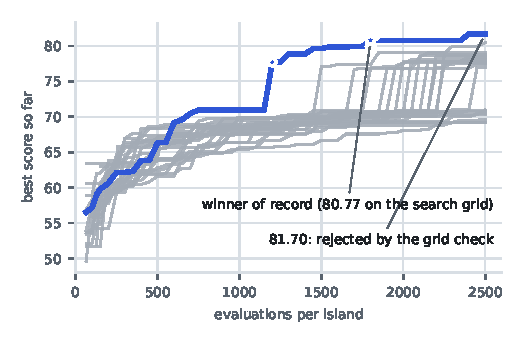
\includegraphics[width=\linewidth]{evolution_best.pdf}\\[2pt]
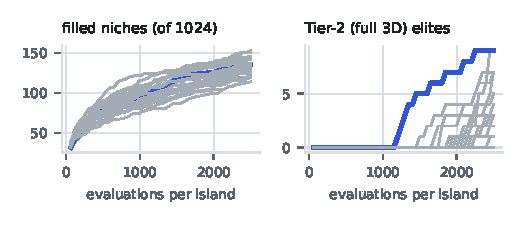
\includegraphics[width=\linewidth]{evolution_archive.pdf}
\caption{Top: best score so far of each island (the winning island in colour; the dot marks its first full-3D
best). Bottom: filled niches and Tier-2 elites per island.}\label{fig:evo}
\end{figure}

\begin{figure*}[t]
\centering
% generated by g3-release-tex: best design of the winning island at each logged checkpoint
\begin{minipage}[t]{0.140\textwidth}\centering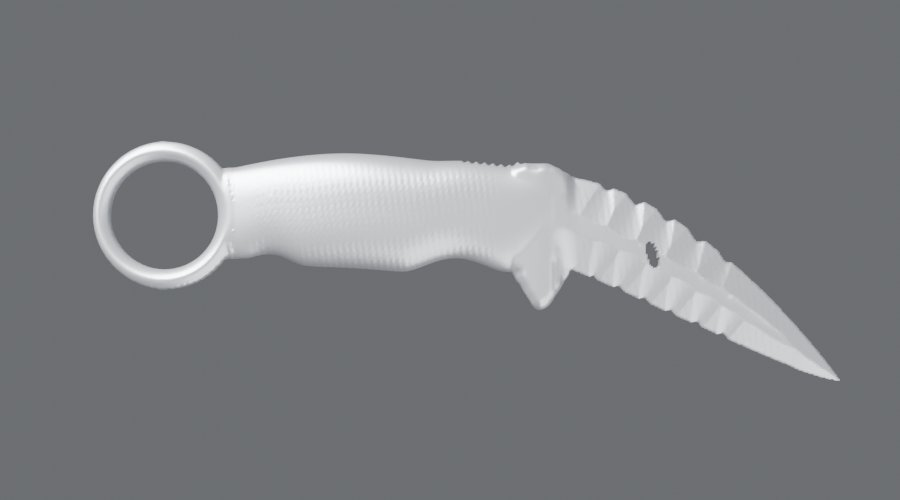
\includegraphics[width=\linewidth]{../../../docs/g3/v3.0.0/img/lineage_00064.jpg}\\[-1pt]{\EItablefont eval 64\\ 56.54, 72.1 g}\end{minipage}\hfill
\begin{minipage}[t]{0.140\textwidth}\centering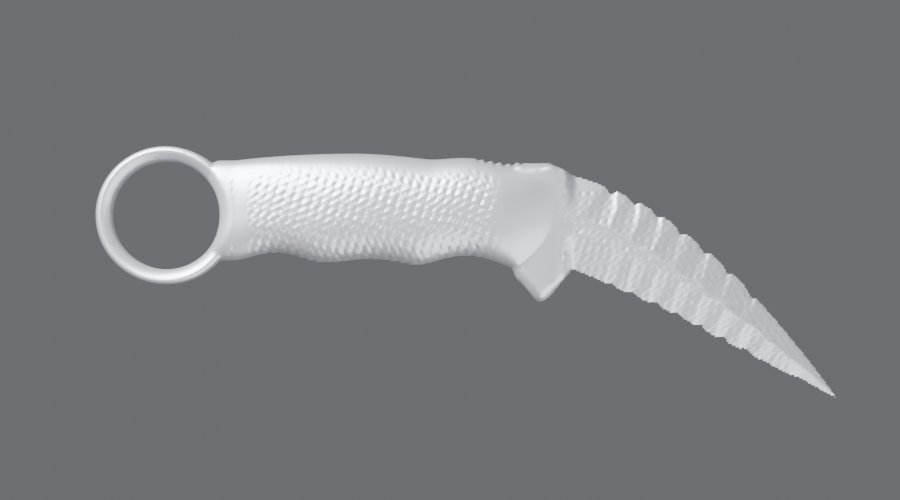
\includegraphics[width=\linewidth]{../../../docs/g3/v3.0.0/img/lineage_00128.jpg}\\[-1pt]{\EItablefont eval 128\\ 59.01, 65.3 g}\end{minipage}\hfill
\begin{minipage}[t]{0.140\textwidth}\centering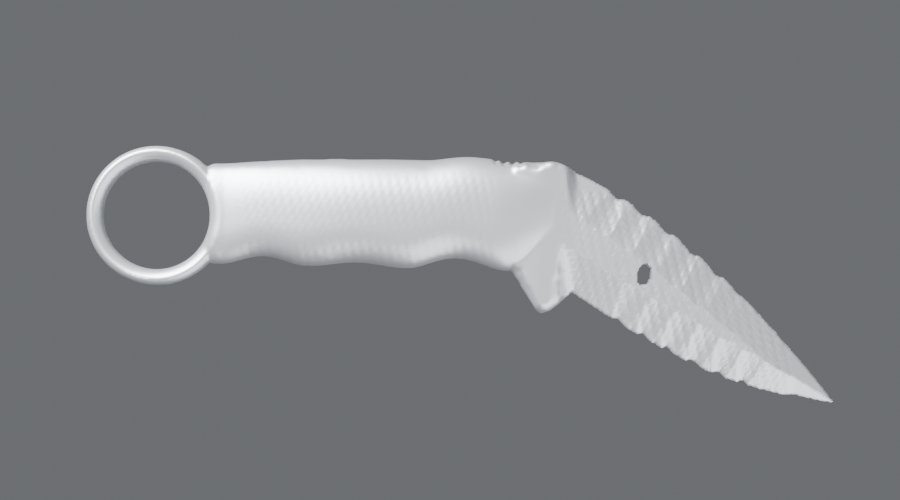
\includegraphics[width=\linewidth]{../../../docs/g3/v3.0.0/img/lineage_00256.jpg}\\[-1pt]{\EItablefont eval 256\\ 62.15, 68.0 g}\end{minipage}\hfill
\begin{minipage}[t]{0.140\textwidth}\centering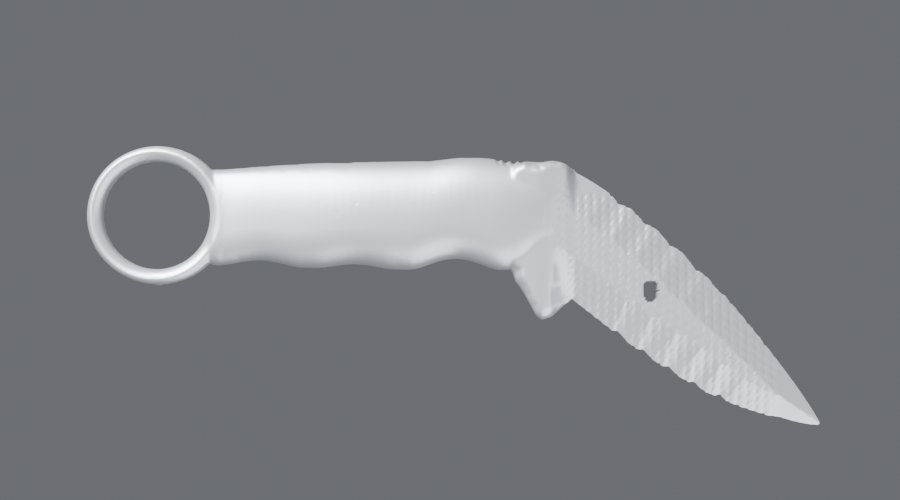
\includegraphics[width=\linewidth]{../../../docs/g3/v3.0.0/img/lineage_00512.jpg}\\[-1pt]{\EItablefont eval 512\\ 66.34, 59.9 g}\end{minipage}\hfill
\begin{minipage}[t]{0.140\textwidth}\centering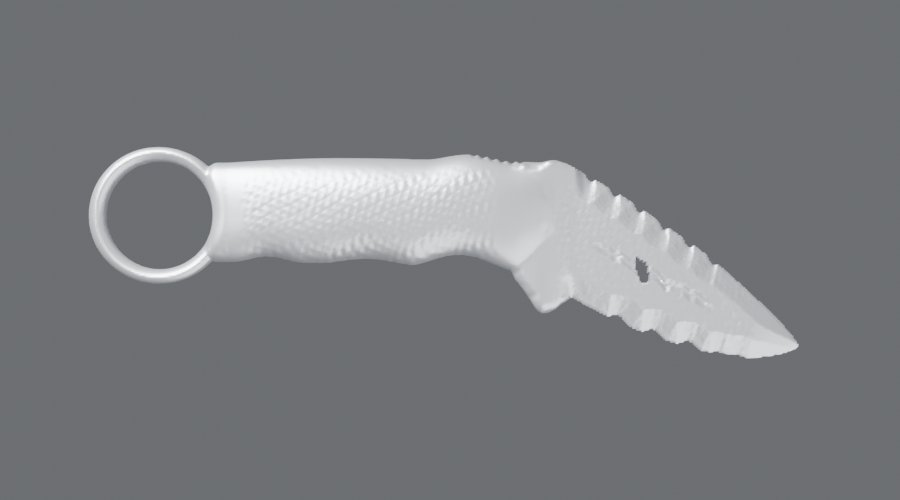
\includegraphics[width=\linewidth]{../../../docs/g3/v3.0.0/img/lineage_01024.jpg}\\[-1pt]{\EItablefont eval 1,024\\ 70.94, 62.4 g}\end{minipage}\hfill
\begin{minipage}[t]{0.140\textwidth}\centering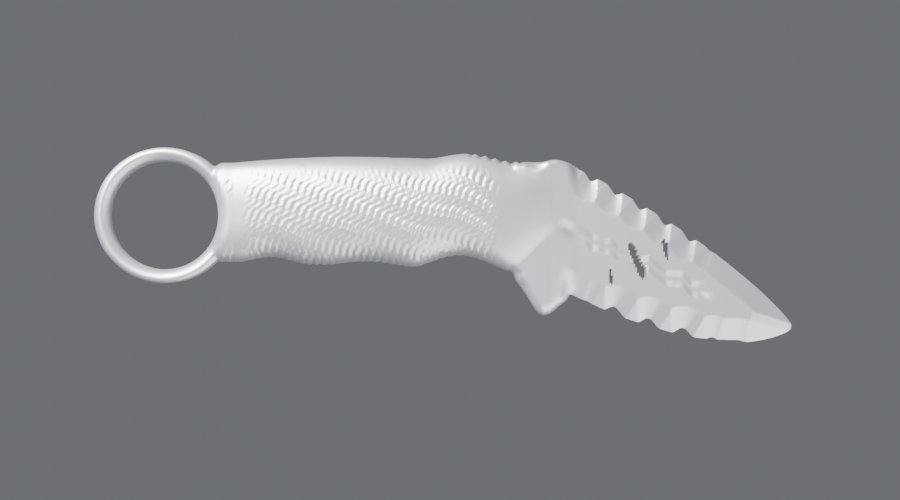
\includegraphics[width=\linewidth]{../../../docs/g3/v3.0.0/img/lineage_02048.jpg}\\[-1pt]{\EItablefont eval 2,048\\ 80.77, 56.0 g\\ \textbf{winner of record}}\end{minipage}\hfill
\begin{minipage}[t]{0.140\textwidth}\centering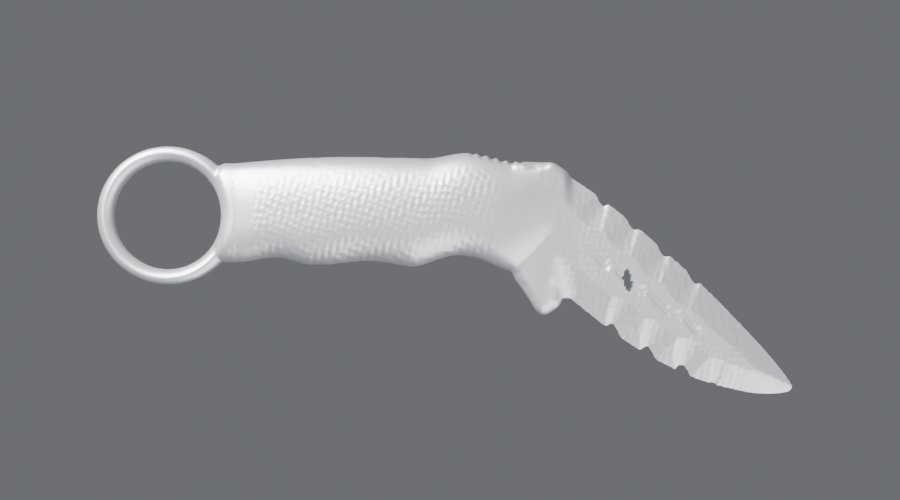
\includegraphics[width=\linewidth]{../../../docs/g3/v3.0.0/img/lineage_02500.jpg}\\[-1pt]{\EItablefont eval 2,500\\ 81.70, 51.3 g\\ \textbf{rejected by the grid check}}\end{minipage}\hfill

\caption{Best design of \gWinIsland{} at each logged checkpoint (a checkpoint sequence, not a parent--child
lineage): evaluation, best score and mass on the search grid. Same camera, light and material for every frame; geometry is the exported mesh.}\label{fig:lineage}
\end{figure*}

\subsection{Choosing the winner on the print grid}
The search measures every design on an $h = \gH$ mm grid, and that grid can undercount mass. The search's own leader,
\gLeader{} (Tier-2 score \gLeaderTierTwo{} at $h = \gH$ mm on the platform of record; the search host logged it a little higher, Fig.~\ref{fig:lineage}), weighs \gLeaderMassA{} g at $h = \gH$ mm but
\gLeaderMassB{} g at $h = 0.2$ mm and \gLeaderMassC{} g at $h = 0.15$ mm, and its Tier-1 score falls from
\gLeaderScoreA{} to \gLeaderScoreB{} (Table~\ref{tab:grid}). The two finest grids agree within \gGridAgree~\% for every design, so the ranking
and the mass of record are measured at $h = \gHRank$ mm, the grid of the print file; the voxel finite-element
check (Section~\ref{sec:measure}) runs at $h = \gFeH$ mm.
The final ranking ordered every elite by its record from the run, re-evaluated the top 32 at Tier 2 at
$h = \gHRank$ mm, and the top 8 again on the platform of record (Table~\ref{tab:top}). The top eight span
\gScore--\gTopLast, a spread the measurement chain does not resolve, so \emph{best} below means first of these eight.

\begin{table}[t]
\caption{Grid check: mass (g) of the top 8 of the search-grid ranking at five voxel pitches $h$ (mm), Tier 1}\label{tab:grid}
\centering
\begin{tabular}{@{}lrrrrr@{}}
\toprule
Design & 0.4 & 0.3 & 0.25 & 0.2 & 0.15 \\
\midrule
\gGridRows
\bottomrule
\end{tabular}
\end{table}

\begin{table}[t]
\caption{Final ranking: Tier 2 at $h = \gHRank$ mm on the platform of record}\label{tab:top}
\centering
\begin{tabular}{@{}rlrr@{}}
\toprule
Rank & Design & Score & Mass (g) \\
\midrule
\gTopEightRows
\bottomrule
\end{tabular}
\end{table}

\begin{figure*}[t]
\centering
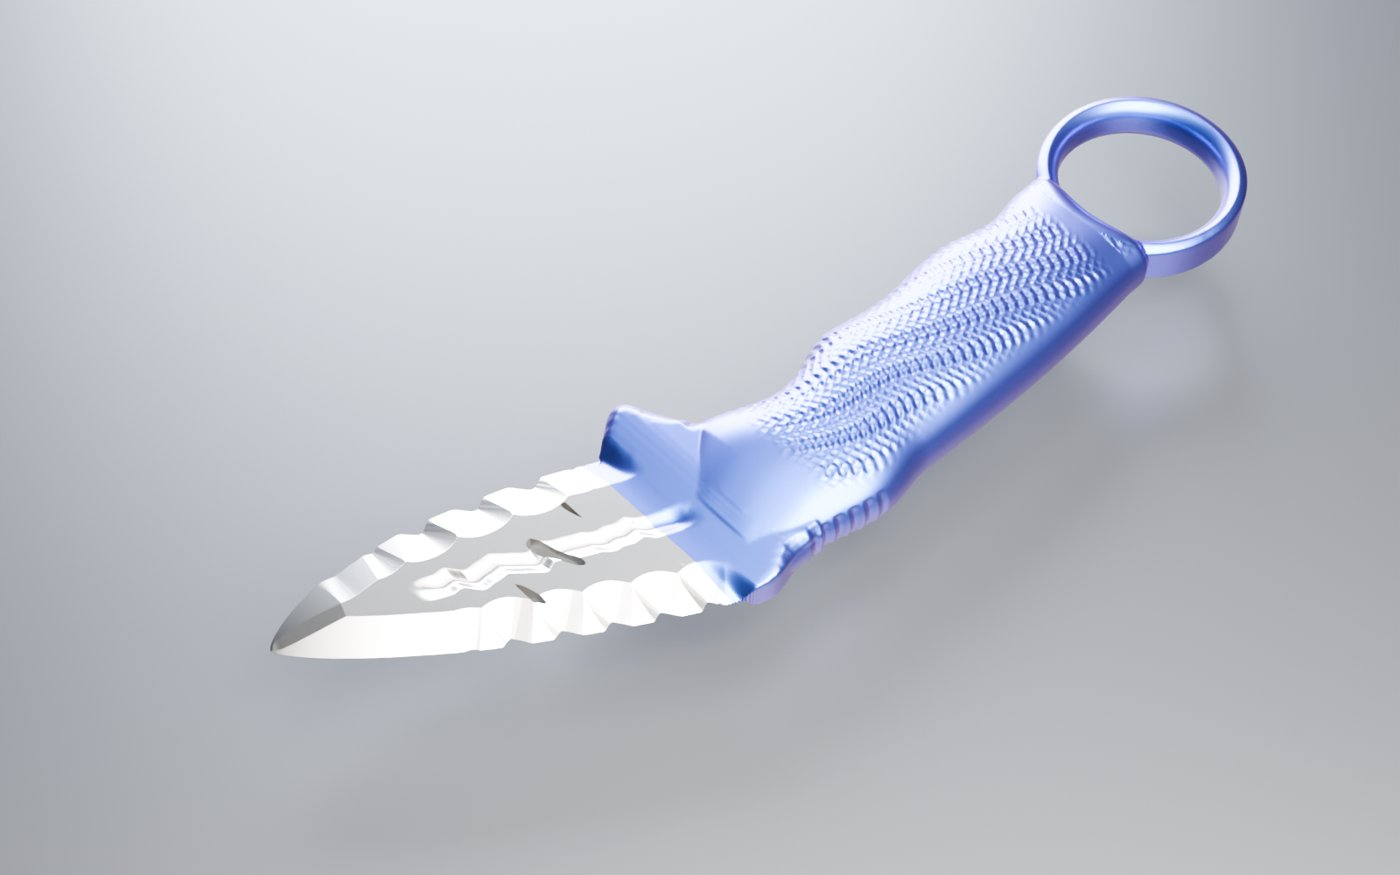
\includegraphics[width=0.49\textwidth]{hero.jpg}\hfill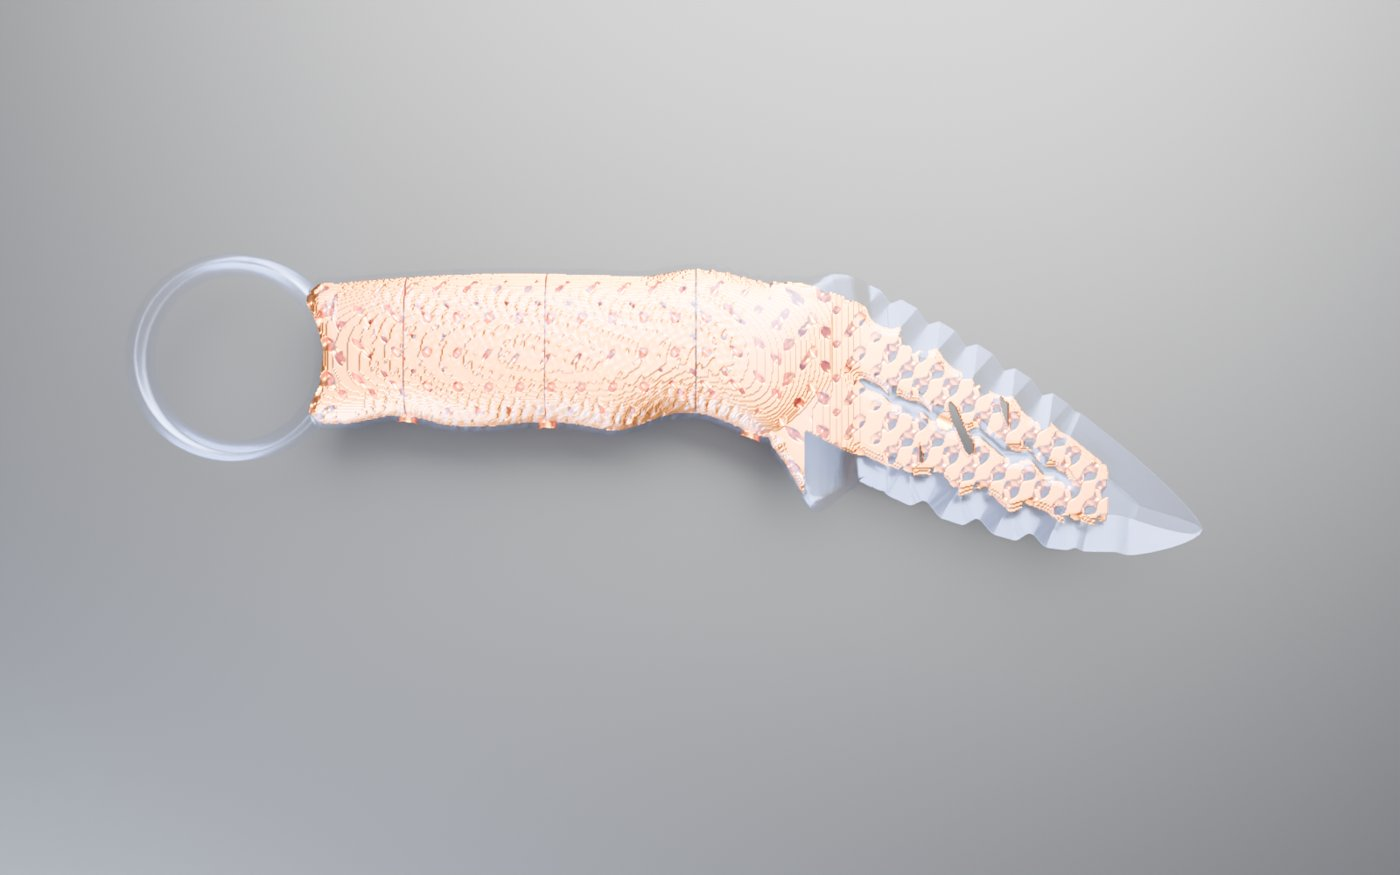
\includegraphics[width=0.49\textwidth]{xray.jpg}\\[3pt]
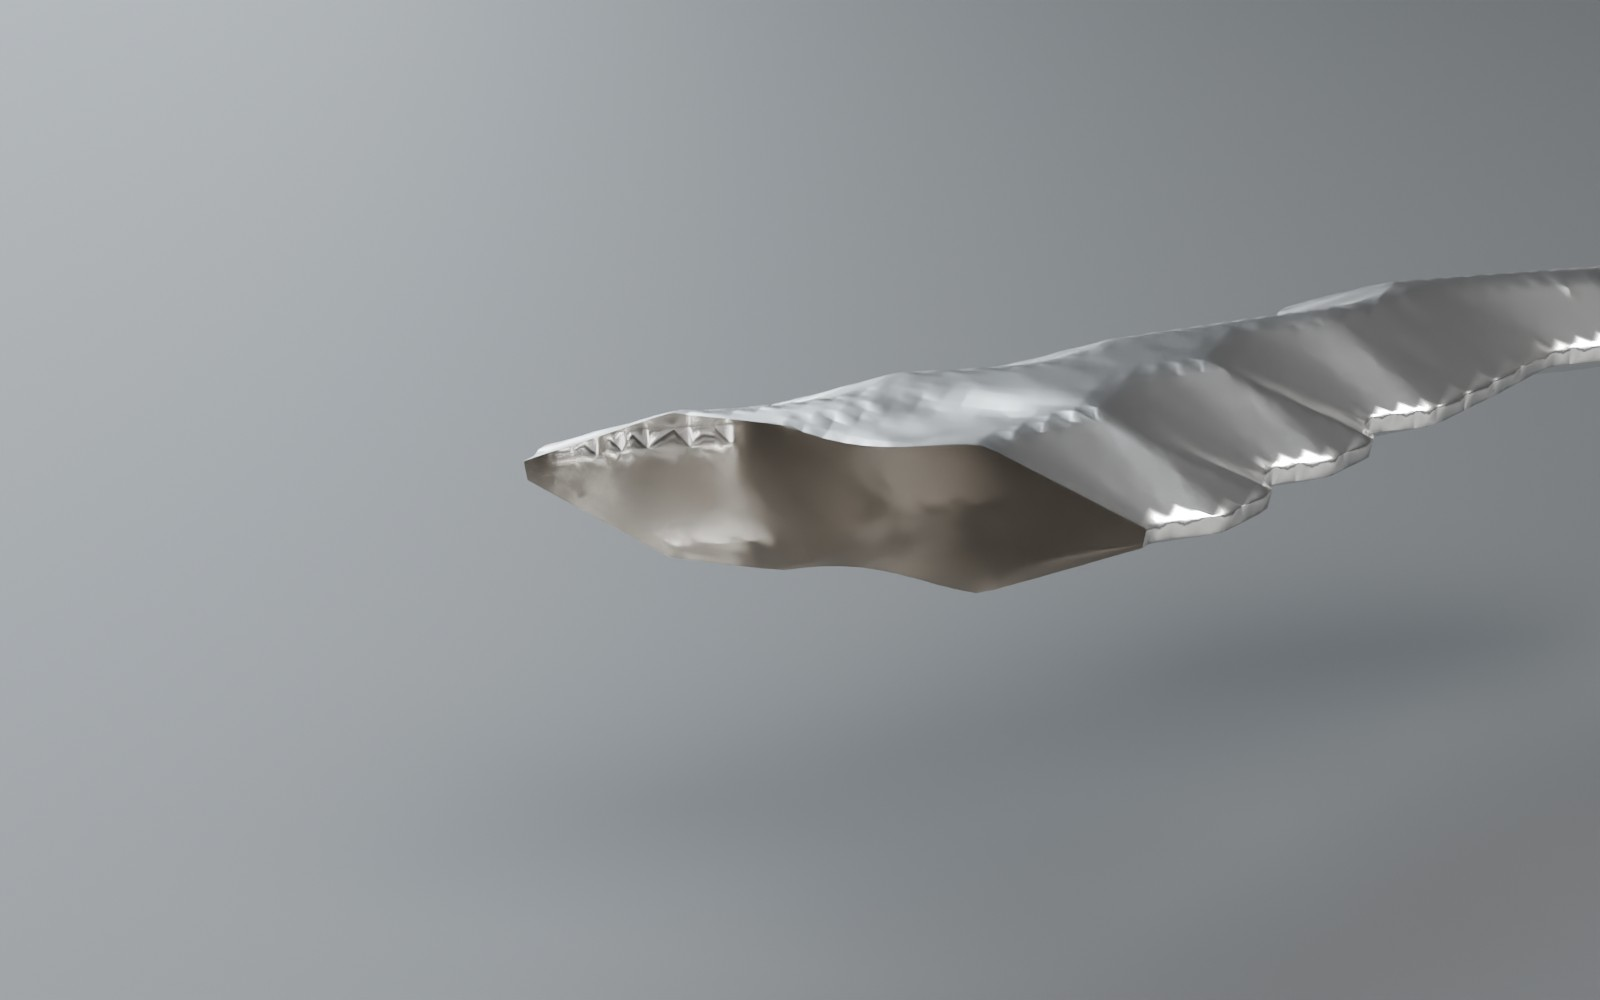
\includegraphics[width=0.32\textwidth]{cut_b.jpg}\hfill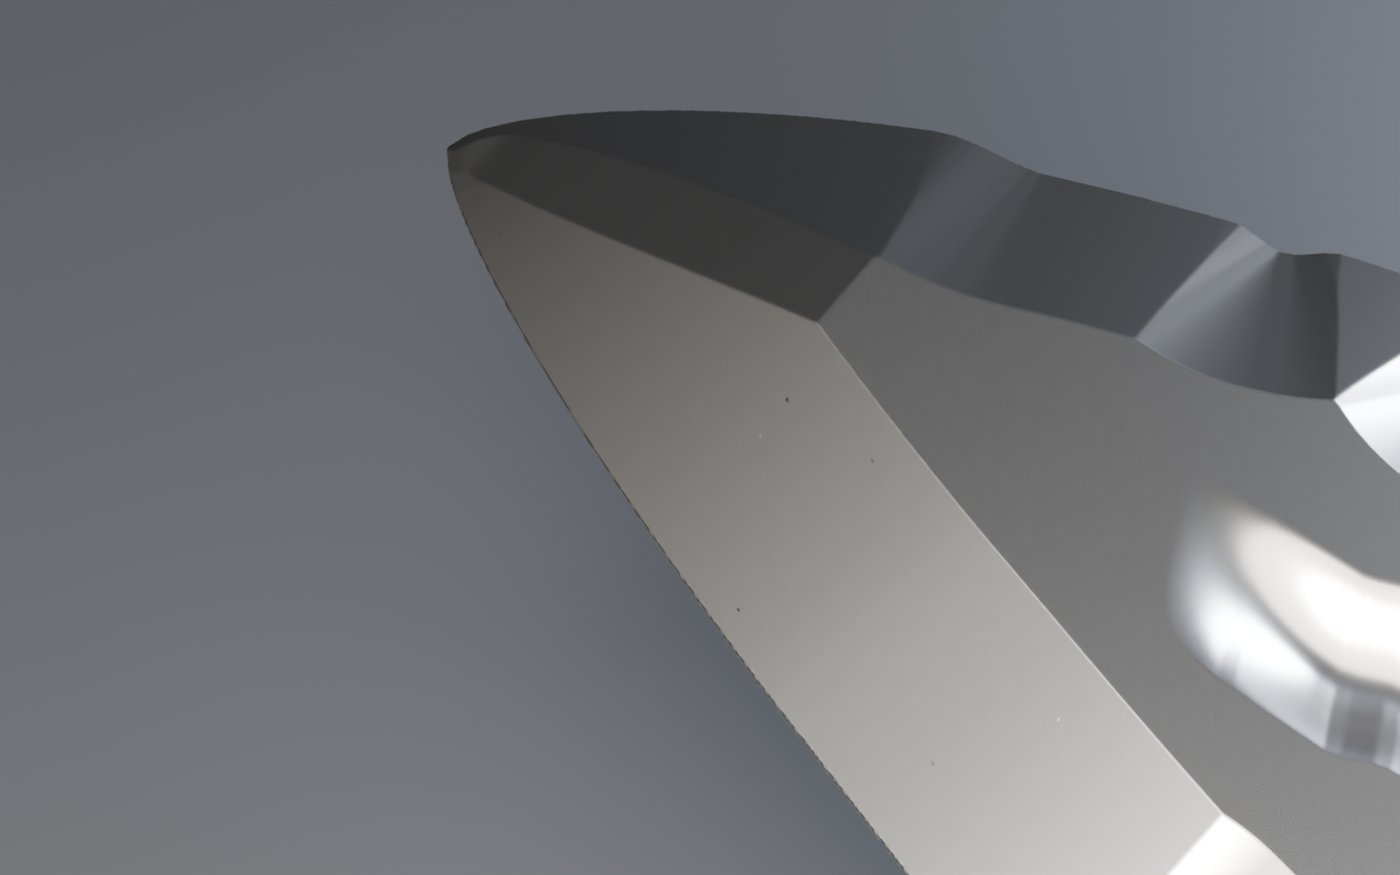
\includegraphics[width=0.32\textwidth]{tip.jpg}\hfill
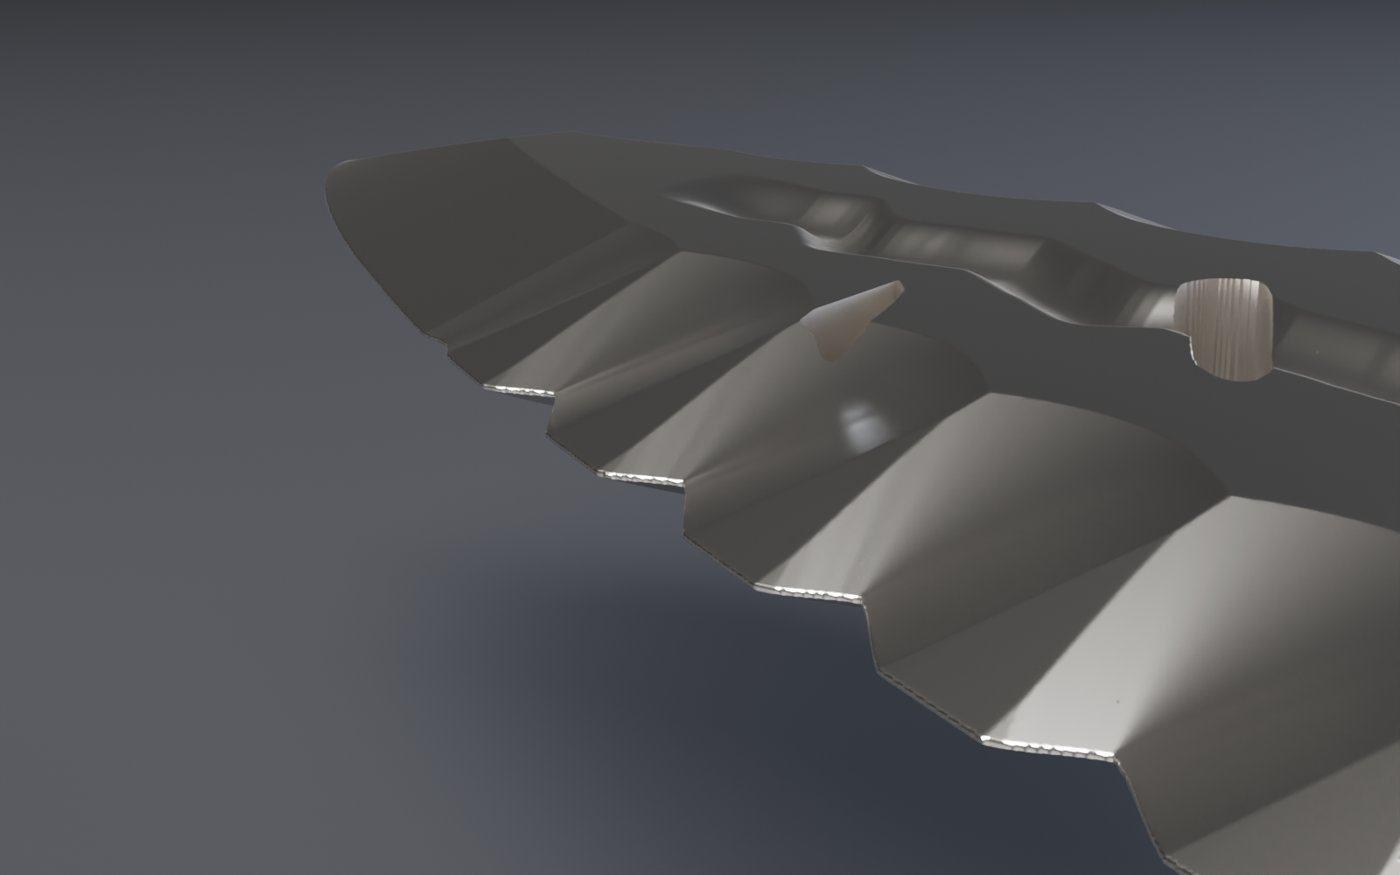
\includegraphics[width=0.32\textwidth]{edge_b.jpg}
\caption{\gDesign. Top: the knife, and an x-ray with every internal cavity in amber. Bottom: a section across the blade
30 mm from the point, the point, and the spine edge with its serrations. Cycles renders of the exported meshes; the blade
is meshed at 0.05 mm from the exact decoder law, the rest at 0.2 mm voxels.}\label{fig:hero}
\end{figure*}

\subsection{The best individual}
The best individual, \gDesign{} (genome hash \gGenomeSha), scores \gScore{} with a weighted base of \gBase{} and an
ergonomic multiplier of \gE. Its grip is \gLg{} mm long with a swell perimeter of \gSwellPerim{} mm and a height-to-width
ratio of \gHoT; the guard is \gGuardH{} mm high and the reach of the blade from the guard is \gReach{} mm. Its print mesh
weighs \gMassG{} g (Table~\ref{tab:mass} lists the four masses of this design). Fig.~\ref{fig:hero} shows it; Table~\ref{tab:best} lists its measurements.

\begin{table}[t]
\caption{Results for the best individual (platform of record; each model as labelled)}\label{tab:best}
\centering
\begin{tabular}{@{}lr@{}}
\toprule
Measure & Value \\
\midrule
Mass, print mesh (watertight, 0.2 mm) & \gMassG{} g \\
Edge A per-side angle, apex / bevel & \gEdgeAApexLo--\gEdgeAApexHi / \gEdgeABevelLo--\gEdgeABevelHi\textdegree \\
Edge B per-side angle, apex / bevel & \gEdgeBApexLo--\gEdgeBApexHi / \gEdgeBBevelLo--\gEdgeBBevelHi\textdegree \\
Grind ends from the point, A / B & \gEdgeATo{} / \gEdgeBTo{} mm \\
Unsharpened plunge, A / B & \gEdgeAPlunge{} / \gEdgeBPlunge{} mm \\
Serration depth, A / B & \gEdgeADepth{} / \gEdgeBDepth{} mm \\
Scallops, A / B & \gEdgeATeeth{} / \gEdgeBTeeth \\
Weakest tooth SF, A / B (teeth checked) & \gEdgeAToothSF{} / \gEdgeBToothSF{} (\gEdgeATeethChecked{} / \gEdgeBTeethChecked) \\
Solid tip SF (1.82 N$\cdot$m twist) & \gTipSF \\
Lateral capacity (search plate mesh) & \gLatN{} N \\
Grip SF, worst of four cases (formula) & \gGripSF \\
Human-max twist SF (search plate mesh) & \gHmTwist \\
Spine 3427 N SF (search plate mesh) & \gHmSpine \\
Ring bearing / back capacity & \gRingBear{} / \gRingBack{} N \\
Fatigue SF / yield-sequence ratio (as coded) & \gFat{} / \gSeq \\
Buckling factor $\lambda$ (analytic) & \gBuck \\
\bottomrule
\end{tabular}
\end{table}

\subsection{Diagnostics added in v3.0.3}\label{sec:diag}
Four diagnostics re-examine this design without changing its receipt or the ranking (\code{g3-diagnostics};
\code{evidence/g3/v\gRecord/diagnostics/}).
\begin{itemize}
\item \textbf{Yield sequence per load case.} The ratio in Table~\ref{tab:best} divides the grip's worst safety factor,
set by the spine load, by the blade's under the 260~N lateral load, so it mixes two load cases. Taken per case with the
voxel-FE grip factors, the ratios are \gSeqLat{} (lateral), \gSeqTwist{} (twist) and \gSeqSpine{} (spine); only the spine
case is below 1.2.
\item \textbf{Fatigue.} The coded fatigue stress divides the plate peak by the thin-wall knock-down \gJointK{} that the
allowable already carries. Applied once, the factor is \gFatCorr{} instead of \gFat.
\item \textbf{Solid tip.} The thickness raster fed to the TET10 model is filled at cell corners and read at cell
centres, a half-cell offset. With the offset removed, the production mesh gives \gTipRaster{} instead of \gTipSF. The
point is blunt in plan view: its included angle is \gTipAngleOne, \gTipAngleTwo{} and \gTipAngleThree\textdegree{} at
1, 2 and 3~mm from the point (\gTipWidthTwo~mm wide at 2~mm), which the thickness-only point gate does not measure.
\item \textbf{Plate model.} Refining the search's blade plate mesh to maximum element areas of \gPlateAreaA,
\gPlateAreaB, \gPlateAreaC{} and \gPlateAreaD~mm$^2$ gives lateral capacities of \gPlateLatA, \gPlateLatB, \gPlateLatC{}
and \gPlateLatD~N. The series does not converge, as a peak stress at sharp features does not, so the plate's lateral,
twist and spine values are values of the search model, not converged estimates.
\item \textbf{Mass.} Table~\ref{tab:mass} lists the four masses of the design. Scored at its print-mesh mass it would
score \gScoreAtMesh{} instead of \gScore. The grip holds \gZoneGripPct~\% of the printed mass, the blade
\gZoneBladePct~\% and the ring \gZoneRingPct~\%.
\end{itemize}

\begin{table}[t]
\caption{The four masses of the best individual}\label{tab:mass}
\centering
\begin{tabular}{@{}lr@{}}
\toprule
Definition & Mass (g) \\
\midrule
Search voxel count, $h = \gH$ mm & \gMassVoxelG \\
Ranking voxel count, $h = \gHRank$ mm (scored) & \gMassRankG \\
Print mesh, watertight, 0.2 mm (of record) & \gMassG \\
Upload mesh in \code{cad/} (coarser, under 50 MiB) & \gMassUploadG \\
\bottomrule
\end{tabular}
\end{table}

\begin{figure}[!t]
\centering
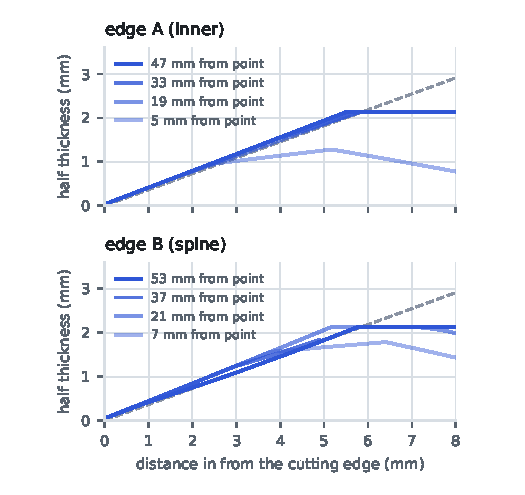
\includegraphics[width=\linewidth]{edge_sections.pdf}
\caption{Upper half of the blade section at four stations of each edge, true scale, against a 20\textdegree{} per-side
grind (dashed). Profiles stop where a lightening slot begins.}\label{fig:edges}
\end{figure}

\subsection{Edges and serrations}
Fig.~\ref{fig:edges} plots the blade section at four stations of each edge, measured along the true edge normal with the
exact decoder law. Every station of an edge lies on one line: edge A at \gEdgeAApexLo--\gEdgeAApexHi\textdegree{} per side
and edge B at \gEdgeBApexLo--\gEdgeBApexHi\textdegree, with no slope steeper than \gEdgeASteep\textdegree{} and
\gEdgeBSteep\textdegree{} within 2 mm of the edge. Both edges are serrated over the rear part of the blade, and the
grinds run on through the plain point region to \gEdgeATo{} and \gEdgeBTo{} mm from the point. Of the teeth between scallops (\gEdgeATeethChecked{} on edge A and \gEdgeBTeethChecked{} on edge B), the weakest has a
safety factor of \gToothMin{} under the \gToothSnag{} N snag and \gToothPry{} N pry, which \gToothReading{} of 1; the end
tooth of each span, bounded by a scallop on one side only, is not checked.

\section{Limits of the result}\label{sec:limits}
\begin{eibox}{What this result is not}
It is a computational design. Nothing has been printed, heat-treated, sharpened or tested, and no safety factor here is
a qualification.
\end{eibox}
\begin{itemize}
\item \textbf{Strength against the targets.} Against a target of 1, the solid tip (\gTipSF) \gTipReading; the grip under
the spine load (worst of four cases by the beam formula \gGripSF; spine load by voxel FE \gFeGripSpine) \gGripReading; the human-maximum twist (plate \gHmTwist, voxel FE
\gFeRootTwist) \gTwistReading; fatigue (\gFat) \gFatReading; and the yield-sequence ratio (\gSeq{} against 1.2)
\gSeqReading. Lateral capacity \gLatReading{} and the ring \gRingReading.
\item \textbf{Mass.} The design weighs \gMassG{} g, which \gMassReading.
\item \textbf{Assumed loads.} The tooth snag and pry loads are conservative research assumptions, not measured use loads.
The buckling factor is an analytic lateral-torsional estimate~\cite{timoshenko1961}, not an eigenvalue solve.
\item \textbf{Models.} Voxel finite elements resolve the printed geometry only to $h = \gFeH$ mm and report percentiles,
not peaks; the plate and beam surrogates of the search differ from them (Table~\ref{tab:fe}). Surfaces come from marching
tetrahedra on the voxel SDF~\cite{doi1991}, except the blade, which is re-meshed at 0.05 mm from the exact decoder law
with marching cubes~\cite{lorensen1987}. Two objective terms are held fixed or capped in this release
(Section~\ref{sec:objective}), and the buckling factor is an analytic estimate.
\item \textbf{Coarse search grid.} The archive was selected at $h = \gH$ mm, which undercounts the mass of some
designs (Table~\ref{tab:grid}); only the final ranking is measured at $h = \gHRank$ mm, so designs that the coarse grid
scored low were never re-checked.
\item \textbf{One shortened cohort.} The release cohort is \gEvalsIsland{} evaluations per island on one host; another
seed or a longer run may find a better design.
\end{itemize}

\section{Reproducibility}\label{sec:repro}
The release is commit \gCommit{} with decoder hash \gDecoder. The winner's 179-gene row is
\code{evidence/g3/v\gVersion/winner_genome.csv}; every island's logged history, the ranking records, the edge profile,
the blade facts and the finite-element results sit next to it under \code{evidence/g3/v\gVersion/}, listed with their
SHA-256 in \code{SHA256SUMS}. The receipt \code{release.json} is the single source of this paper and of the repository
README: \code{g3-release-tex} turns it into the macros used here, and \code{ops/ci/gen\_readme.py} into the README. The
cohort is reproduced by building \code{g3-evolve} at that commit and running each island with its seed, \code{--h
\gH}, \code{--tier1-gate \gGateOne}, \code{--tier2-gate \gGateTwo} and \code{--log-every 50}; \code{pilot\_tools export}
rebuilds the watertight envelope and print mesh from the genome row. The binary STL files (millimetres) are listed in
Table~\ref{tab:assets}.

\begin{table}[t]
\caption{CAD files of the best individual (binary STL, millimetres; each file name starts with the design identifier)}\label{tab:assets}
\centering
\begin{tabular}{@{}p{0.40\linewidth}rrl@{}}
\toprule
File & Triangles & MiB & Where \\
\midrule
\gAssetRows
\bottomrule
\end{tabular}
\end{table}

\section{Conclusion}
Putting the edge and serration rules into the decoder made every design the search could express a knife with a
correctly ground, double-serrated two-sided blade, and the search then traded mass, strength and ergonomics within that
space. The search also exposed a gap in the measurement chain: on its coarse grid, a design could look lighter
than it would print. Re-measuring the ranking on the print grid closed that gap for this release. The best individual of
the release, \gDesign, scores \gScore{} at \gMassG{} g with an ergonomic multiplier of \gE. The limits in
Section~\ref{sec:limits} set the next work: a stronger sharp point, a stiffer hollow grip under the spine load, a search
grid fine enough that it cannot be gamed, and a longer cohort, all measured the same way.


\begin{thebibliography}{9}
\bibitem{mouret2015} J.-B. Mouret and J. Clune, ``Illuminating search spaces by mapping elites,'' \emph{arXiv:1504.04909}, 2015.
\bibitem{vassiliades2018} V. Vassiliades, K. Chatzilygeroudis, and J.-B. Mouret, ``Using centroidal Voronoi tessellations to scale up the multidimensional archive of phenotypic elites algorithm,'' \emph{IEEE Trans. Evol. Comput.}, vol. 22, no. 4, pp. 623--630, 2018.
\bibitem{joe2008} S. Joe and F. Y. Kuo, ``Constructing Sobol sequences with better two-dimensional projections,'' \emph{SIAM J. Sci. Comput.}, vol. 30, no. 5, pp. 2635--2654, 2008.
\bibitem{matousek1998} J. Matou\v{s}ek, ``On the $L_2$-discrepancy for anchored boxes,'' \emph{J. Complexity}, vol. 14, no. 4, pp. 527--556, 1998.
\bibitem{lorensen1987} W. E. Lorensen and H. E. Cline, ``Marching cubes: A high resolution 3D surface construction algorithm,'' \emph{Comput. Graph.}, vol. 21, no. 4, pp. 163--169, 1987.
\bibitem{inglis1913} C. E. Inglis, ``Stresses in a plate due to the presence of cracks and sharp corners,'' \emph{Trans. Inst. Naval Archit.}, vol. 55, pp. 219--241, 1913.
\bibitem{timoshenko1961} S. P. Timoshenko and J. M. Gere, \emph{Theory of Elastic Stability}, 2nd ed. New York: McGraw-Hill, 1961.
\end{thebibliography}
\end{document}
